\chapter{Summary}
Wicked problems like those identified as Millennium Development Goals by the United Nations require an innovative approach for analysis and solution development \citep{UnitedNations2015}. The characteristics of wicked problems, including no definitive problem formulation, no one solution to the problem, conflicting objectives, and no right to be wrong \citep{Rittel1973}. These problems, therefore, are characterized by a level of uncertainty greater that that which can be addressed with simple probabilities or statistics known as deep uncertainty. And these deeply uncertain problems demand new methods of analysis that go beyond a traditional predict-then-act format which seeks a single optimal solution. Instead of seeking the optimal solution, these new methods focus on finding a set of robust solutions that balance conflicting objectives and perform well under a variety of possible futures. 

Several methods have been developed that aim to do just that, identified in this thesis as robust decision support methods, several methods of which were developed following the structure of robust decision making, introduced by \citep{Lempert2002}. Each method developed takes its own approach to determining a set of robust policy alternatives to decision makers. The choice of which method to use, therefore, will have a significant impact on the results of analysis for both decision makers and policy analysts.  Though there has been some work to compare the efficacy of these methods, no structured comparative framework has been developed that supports the fair comparison of multiple methods of robust decision support. Furthermore, despite the fact that method performance is likely largely dependent on the problem and policy implementation structure, existing comparative literature has consistently made use of a single problem and policy structure. 

\vspace{\baselineskip}
{\Large {\color{title}Goal of Research}}
\vspace{0.5\baselineskip} \newline
To that end, the following research question will be addressed: 

\begin{researchquestion}{Research Question}
    What are the trade-offs between different methods of decision support when considering a wicked problems and varying policy implementation structures? 
\end{researchquestion}

This thesis is proposing a well structured comparative framework that supports a fair comparison of robust decision support methods when considering a wicked problem with multiple types of policy implementation structures. Comparison metrics include those related to the setup of the required models and method implementations, how and when each method communicates results of an analysis, and comparison of the results themselves (including robustness of recommended policies and computational cost of execution). 

\vspace{\baselineskip}
{\Large {\color{title}Methods Considered}} 
\vspace{0.5\baselineskip} \newline
This framework is then utilized to compare the efficacy of three robust decision support methods: MORDM, multi-scenario MORDM, and MORO. To support comparison of these methods, a common structure was established that is strongly rooted in the robust decision making structure \citep{Lempert2006}. This structure, visualized in \cref{fig:diff-flows-summary}, highlights the variation between the three methods, which lies in the policy alternative determination step. 

\begin{figure}[ht]
    \centering
    \captionsetup{justification=centering}
    
    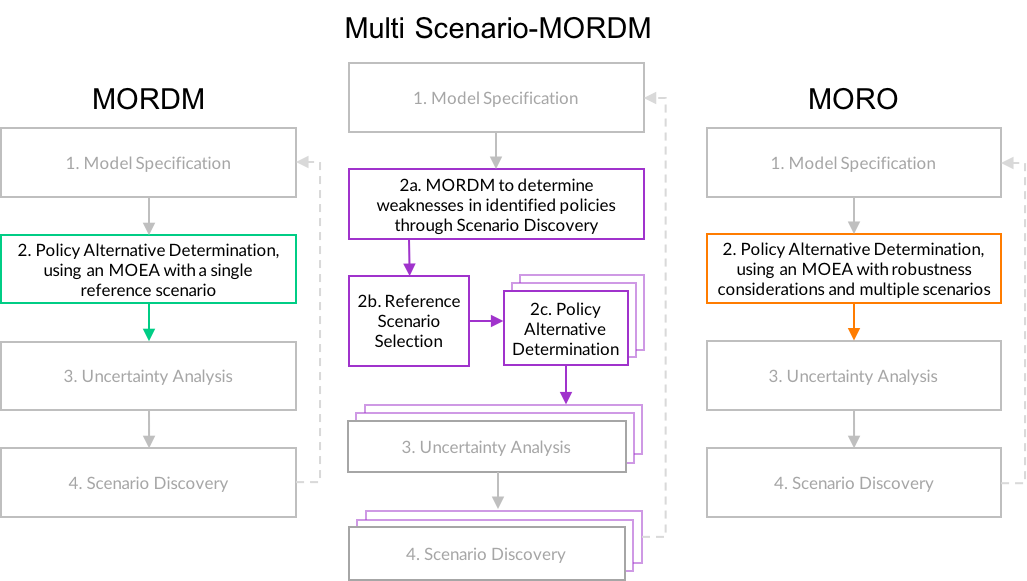
\includegraphics[width=\textwidth]{diff-flows}
    \caption{Comparison of robust decision support framework structures}
    \label{fig:diff-flows-summary}
\end{figure}

The policy alternative determination step in each of the three methods uses a common multi-objective evolutionary algorithm (MOEA) to build a library of potentially robust policy alternatives that will be studied further in the remaining steps of analysis. This thesis uses an algorithm called auto-adaptive $\epsilon$-NSGAII, an innovative MOEA that combines the best features of traditional $\epsilon$-NSGAII, a generational structure and epsilon dominance, with the strongest elements of Borg: auto-adaptive operator selection and adaptive population sizing.

Auto-adaptive $\epsilon$-NSGAII uses evolutionary search techniques to find potentially robust combinations of decision lever values. The fitness of these potential policies is compared using a comparison mechanism, with the alternatives that are not Pareto dominated being added to a set of policies which approximates the Pareto front of the decision lever space. This comparison mechanism is the element of each method that makes it unique. The other elements of each method, including model specification, MOEA parameterization, uncertainty analysis, and scenario discovery, are common to all three methods. 

MORDM uses a single reference scenario to compare the performance of potential policy alternatives, which is generally established with input from decision makers. Multi-scenario MORDM uses a set of reference scenarios that were selected from the vulnerable uncertainty space identified by scenario discovery in a traditional MORDM analysis. The search for alternatives is then run independently for each selected reference scenario. In this way, multi-scenario MORDM attempts to incorporate robustness into the search process. And finally, MORO directly considers robustness of potential policy alternatives by comparing the fitness of policies based on their robustness, calculated with the performance of a policy against a small ensemble of scenarios. 

\vspace{\baselineskip}
{\Large {\color{title}Problem and Policy Structures Considered}}
\vspace{0.5\baselineskip} \newline
The efficacy of each method was tested using a commonly referenced and highly stylized environmental planning problem called the shallow lake problem. 

Three variations of the lake problem are used, which provides the opportunity to compare the efficacy of each method given a wide range of policy structures. The first, labeled intertemporal, represents a static structure, where a predetermined set of decision levers equal to the number of time steps considered (100 in this study) that specifies the anthropogenic pollution released in each time step. The second, direct policy search (DPS), represents the other extreme, a highly adaptive policy structure that updates the anthropogenic pollution released in a time step based on a function that is parameterized with five decision levers. Both of these structures have established and analyzed previously in literature \citep{Quinn2017,Singh2015,Ward2015}, but are not reflective of real-world policy making. 

This study proposes a third policy implementation structure identified as planned adaptive DPS which attempts to match real-world behaviors more closely. This variation follows the structure of the DPS variation, using a function to determine anthropogenic pollution levels, but uses that function to update the amount of anthropogenic pollution after every 10 time steps, instead of after every time step. In this way, the planned adaptive DPS variation better approximates the slower pace of real-world policy structures, which rarely support decision changes every time step due. 

\vspace{\baselineskip}
{\Large {\color{title}Summary of Findings}} 
\vspace{0.5\baselineskip} \newline
The comparison framework establishes eleven points of comparison, and each were considered in the analysis of the results of the 9 pairings of model variation and method. As each of these methods are based on the same RDM structure and share a common robustness definition, many of the comparison metrics did not reveal any differences, especially with respect to model setup, and communication of results and robustness. The variance in comparison mechanisms for the MOEA-based search gives multi-scenario MORDM analysis much more complicated setup requirements, as the set of reference scenarios requires a full MORDM analysis and exhaustive search to find a series of maximally diverse scenarios. 

An analysis of the computational cost indicates that MORO is significantly more cost intensive than the other two methods as a result of the comparison mechanism used, creating significant runtime constraints when compared to the other two robust decision support methods. 

Generally, mean robustness per outcome of interest in \cref{fig:summary-robust-heatmap-mean} shows that for the more robustness is incorporated into the comparison mechanism of the search for potentially robust policy alternatives, the higher the robustness is for the final identified set of alternatives. The exception is for the newly proposed planned adaptive variation and multi-scenario MORDM pairing, which produced a set of policy alternatives that prioritized robustness of pollution and reliability and sacrificed utility to the town through a significantly more conservative approach to anthropogenic pollution release. These results indicate the impact that reference scenario selection can have on an analysis. 

Also compared is the size of each set of non-dominated policy alternatives, summarized in \cref{table:summary-pareto-size}. Both MORDM and multi-scenario MORDM based analyses lead to a significantly larger number of non-dominated policies that must then be considered throughout the remaining steps of analysis. Methods that recommend larger sets of policy alternatives can prove to be more difficult for decision makers to digest in order to reach a final plan of action. 

\begin{table}[b]
    \centering
    \captionsetup{width=0.85\textwidth}
    \caption[Size of non-dominated policy alternative sets]{Size of the Pareto non-dominated set of policy alternatives for each pairing.}
    \label{table:summary-pareto-size}
    
    \rowcolors{2}{odd-row-blue}{even-row-blue}
    \setlength\arrayrulewidth{1pt}\arrayrulecolor{white}
    \begin{tabularx}{.85\linewidth}{l|r|r|r}
        \rowcolor{tudelft-dark-blue!80}
        & \multicolumn{1}{c|}{\color{white} \textbf{MORDM}}
        & \multicolumn{1}{c|}{\color{white} \textbf{Multi-Scenario MORDM}}
        & \multicolumn{1}{c}{\color{white} \textbf{MORO}} \\ \hline
        
        Intertemporal       & 90    & 291   & 7     \\ \hline
        Planned Adaptive    & 48    & 113   & 6     \\ \hline
        DPS                 & 110   & 209   & 22    \\ \hline
    \end{tabularx}
\end{table}

Reflecting on the research question, this thesis developed a structured comparative framework to compare the effectiveness of multiple methods of robust decision support across multiple policy structure variations for a single deeply uncertain problem. That framework was applied to compare MORDM, multi-scenario MORDM, and MORO, and their efficacy for analysis of multiple variations of the stylized lake problem. A clear trade-off between computational cost and robustness and size of the discovered set of robust alternatives was identified, with MORDM and multi-scenario MORDM producing policy alternatives that are less robust, but with lower computational cost than MORO across lake problem variations. 

\begin{figure}[t!]
    \centering
    \captionsetup{width=0.8\textwidth}
    
    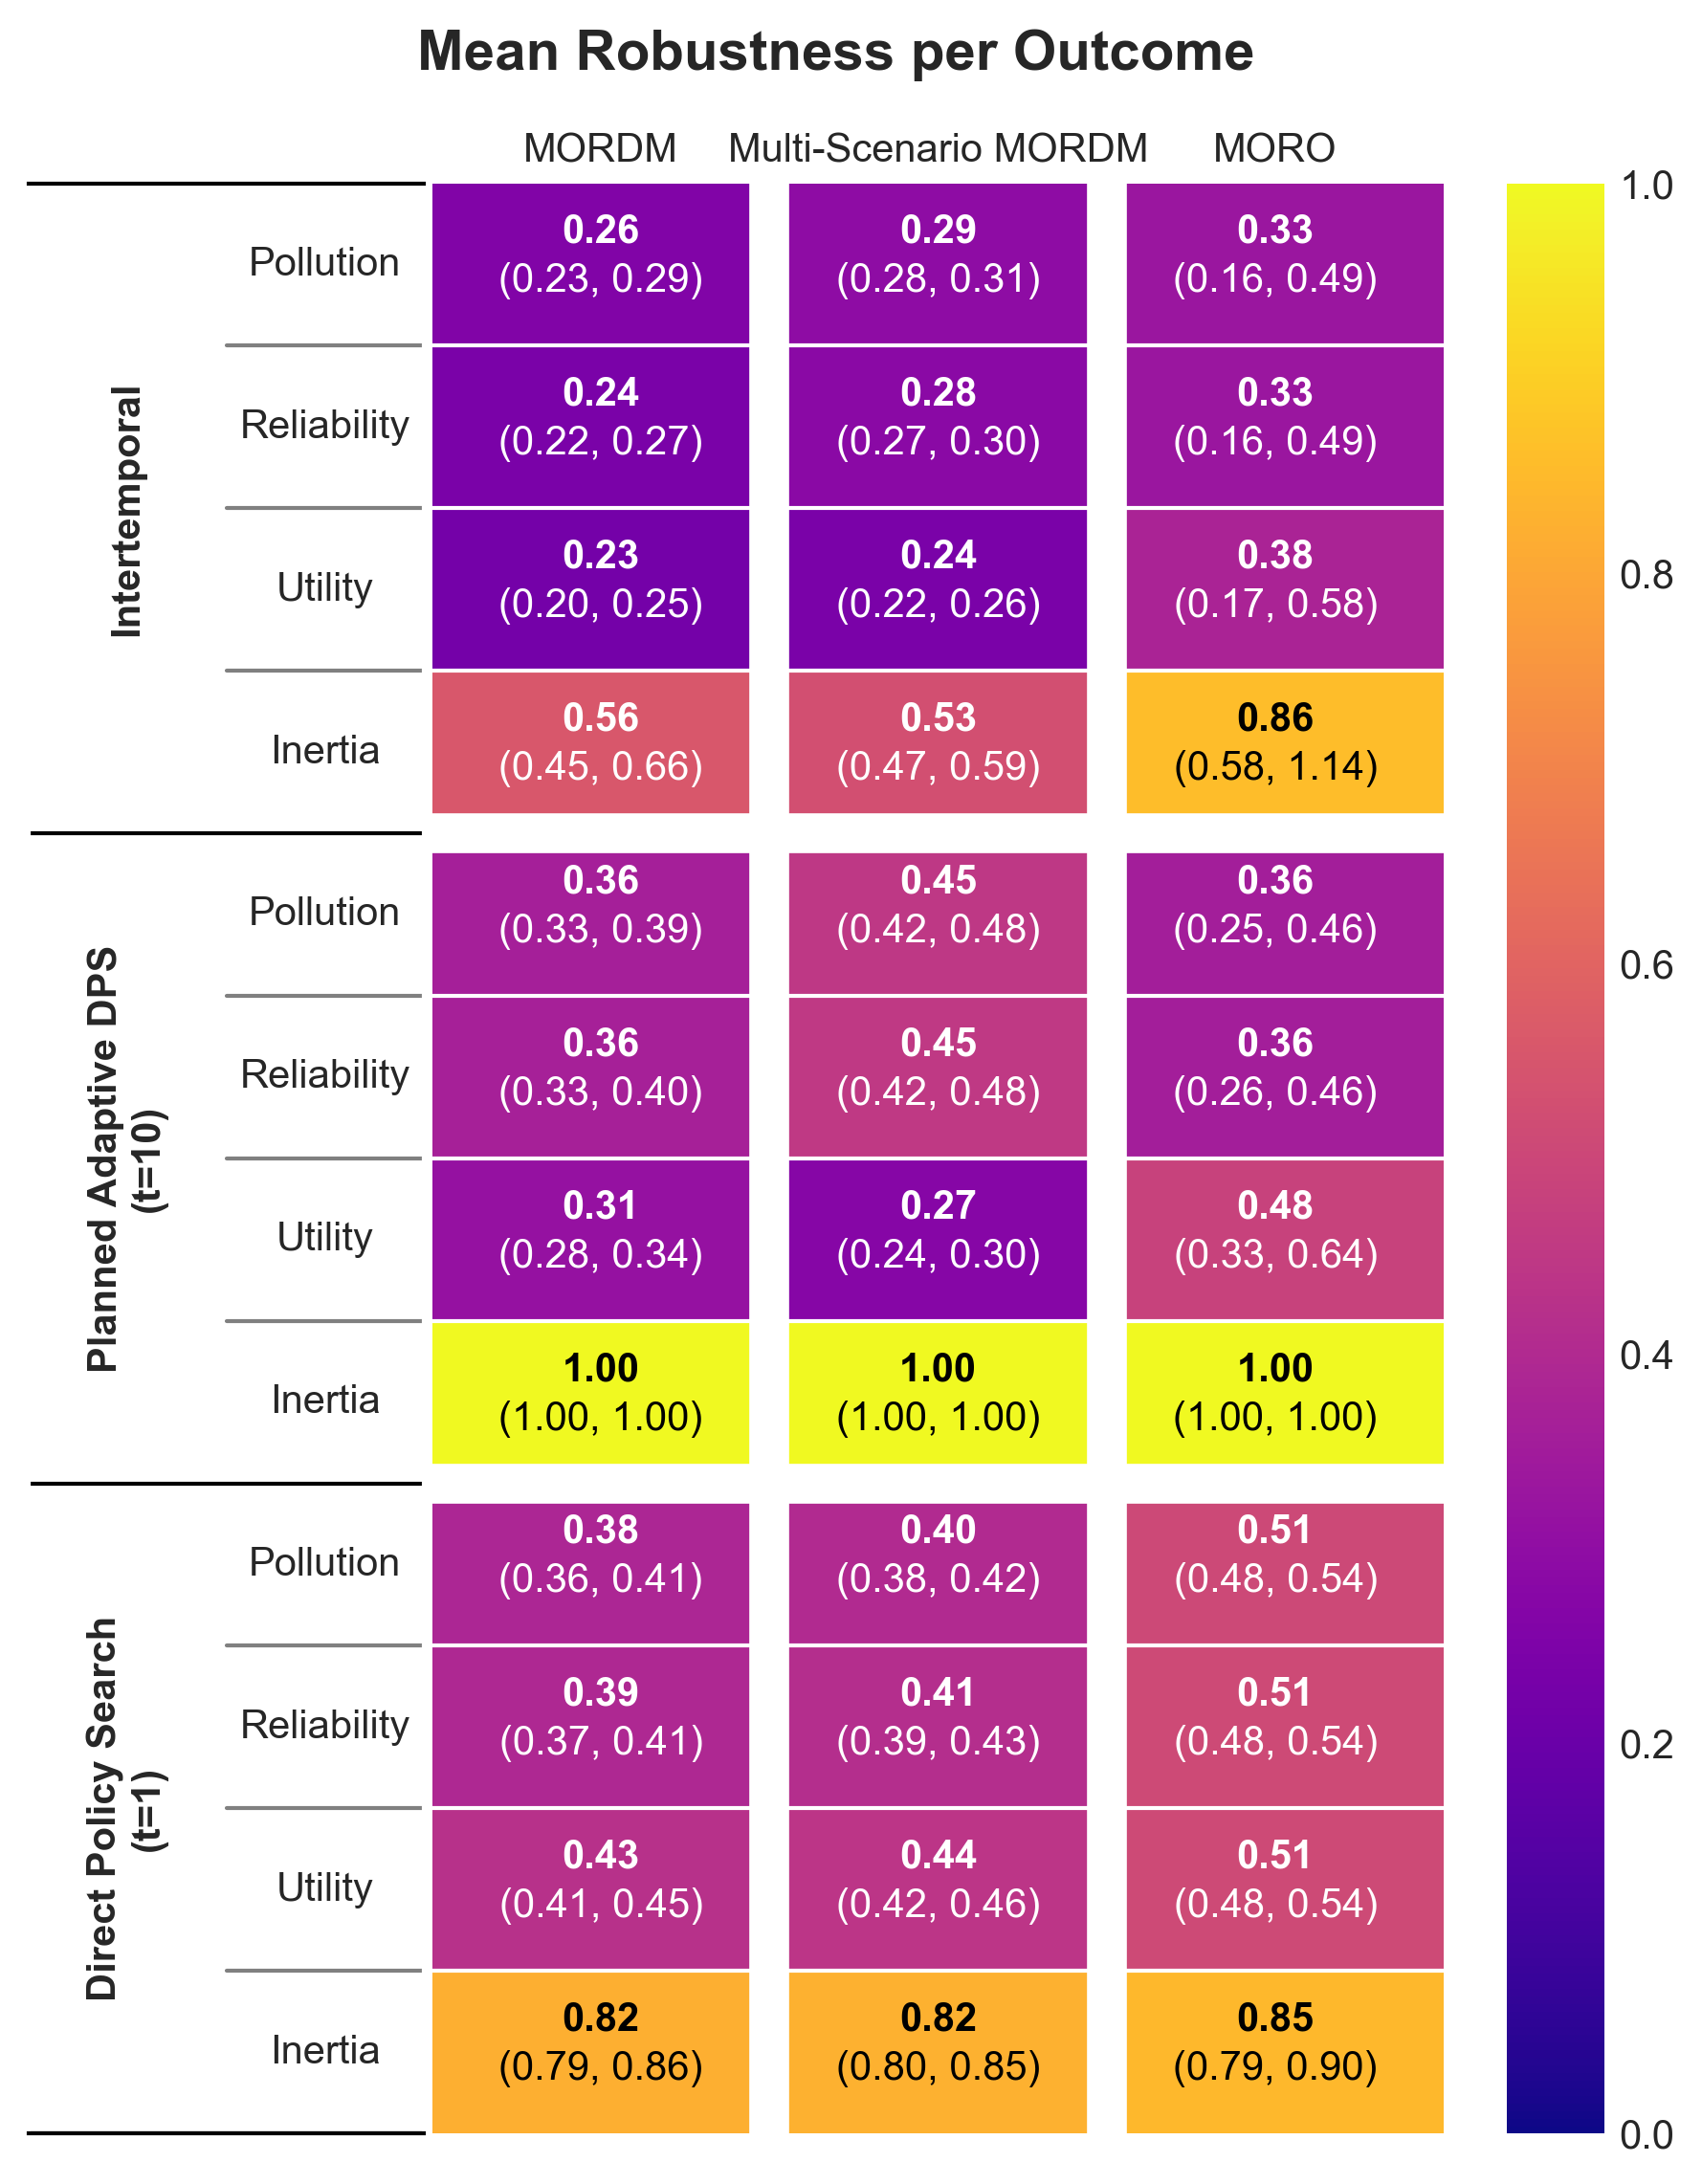
\includegraphics[width=0.8\textwidth]{compare/robust_heatmap_mean}
    \caption[Mean robustness per outcome of interest across all pairings]{Mean robustness per model variation and method pairing. This heat map is annotated to include the bounds of the 95 percent confidence interval surrounding the mean.}
    \label{fig:summary-robust-heatmap-mean}
\end{figure}

Two primary avenues for further research were also identified. First, it may be possible to mitigate the computational cost of MORO by investigating the interplay between the size of the reference scenario set used in optimization, the sampling techniques for that set, and the robustness metric used in an effort to reduce the size of the reference scenario set and therefore computational cost of that method. 

The use of the lake problem represents the second significant avenue of future research. Policy analysis and deep uncertainty literature has relied primarily on this single benchmarking problem to test and compare methods of robust decision making. The development of additional benchmarking problems would benefit both analysts and decision makers, who can leverage new problems to develop a stronger understanding of the efficacy of robust decision support methods than the use of one benchmarking problem can provide alone. 





